\documentclass[conference]{IEEEtran}
\IEEEoverridecommandlockouts
% The preceding line is only needed to identify funding in the first footnote. If that is unneeded, please comment it out.
\usepackage{cite}
\usepackage{amsmath,amssymb,amsfonts}
\usepackage{algorithmic}
\usepackage{graphicx}
\usepackage{textcomp}
\usepackage{xcolor}
\def\BibTeX{{\rm B\kern-.05em{\sc i\kern-.025em b}\kern-.08em
    T\kern-.1667em\lower.7ex\hbox{E}\kern-.125emX}}
\begin{document}

\title{Game Theory. \\ Practical Assignment 2. Report.}

\author{\IEEEauthorblockN{Artem Chernitsa}
\IEEEauthorblockA{\textit{student, group BAI-01} \\
\textit{Innopolis University}\\
Innopolis, Russia \\
a.chernitsa@innopolis.university}
}

\maketitle

\begin{abstract}
This document is a report for the practical assignment on Game Theory course Fall 2022. It includes problem description, theoretical computations, description of proposed solution, important parts of implementation.
\end{abstract}

\begin{IEEEkeywords}
game theory, non-zero-sum games, axelrod's tournament, the prisoner's dilemma, snowball game
\end{IEEEkeywords}

\section{Introduction}
Snowball game is an example of a non-zero-sum game, and axelrod's tournament, which, for understanding, requires a description to understand the nature of this game. In short, two players play against each other on a large field divided into three parts: one for each player and one common zone. Players throw snowballs either onto each other's field, or into a common area where snowballs disappear forever within the game. Every minute a snowball is added to the field with the help of a Snowball Generator Machine (SGM). The goal of each player is to minimize the number of snowballs in their half after 60 minutes. The most important thing is that the players play in the tournament, each with each once, and the rating of each player depends on the total number of remaining snowballs on his half for all the matches played.

\section{Problem Description}

% \subsection{Maintaining the Integrity of the Specifications}

The environment where players play the snowball game is three territorial regions which we will helpfully entitled as A, B, and C fields. Fields A and B contain one player on each side. The field C does not contain any players and should be considered as a hot field where snowballs automatically melt and disappear. The players cannot change their positions and should shot snowballs from the field they are located on. 

Let assume that for both A and B fields the initial number of snowballs is N=100. Each A and B fields have a single SGM. Because of those machines each imaginary minute the number of snowballs N increases by 1 for both fields.

Both players are using special Snowball Cannons (SC) able to shoot snowballs. Assume that shooting does not melt or destroy snowballs. The players can use Cannons at most once per minute to opponent’s field and at most once per minute to hot field (totally at most twice, assume it as sequential shots, where shot to opponent’s field happens firstly). Each shot can contain 1 snowball or more. Not shooting is also allowed and requires 0 to be returned by a proper method. If no shooting happened to opponent’s and hot fields, then it is assumed that during this minute shooting did not happen. If SC was used once or twice per minute, then it is assumed as a presence of shooting during this minute. However, the shooting history affects the maximum number of snowballs shoot for the next minutes. The maximum number of snowballs shoot by cannon per minute (together for both shots) is defined by equation
\begin{equation}
f(x) = \left \lfloor \cfrac{15 \cdot e^x}{15 + e^x} \right \rfloor\label{eq1}
\end{equation}

\section{Theoretical Computations}
\subsection{Calculating Rates}
Since we will have to adjust the strategy depending on the opponent's behavior according to [1], it is necessary to get the maximum available information. To this end, we will first calculate the maximum possible number of snowballs at each waiting interval.

\begin{figure}[htbp]
\centerline{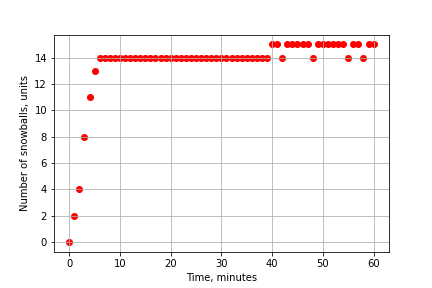
\includegraphics[width=0.5\textwidth]{fig1_maximum_snowball_per_round.png}}
\caption{Dependency the maximum number of snowballs on time t.}
\label{fig}
\end{figure}

As shown in Fig.1 the maximum possible number of balls to throw is 15. However, this amount is reached only after 40 minutes of waiting. Without taking into account SGM, we will be able to throw only 15 balls out of 100. the calculated maximum speeds of throwing snowballs per minute show that the fastest way to throw snowballs is 11 units every 4 minutes. Thus, the speed will be 2.75 snowballs / minute (s/m). For comparison, in Tab.1 all calculated rates are presented.

\begin{table}[htbp]
\caption{Maximum Possible Snowball Rates}
\begin{center}
\begin{tabular}{|c|c|c|}
\hline
\textbf{Snowballs}&\textbf{Interval}&\textbf{Rate, $s/m$} \\
\hline
15& 40& 0.375 \\
\hline
14& 6& 2.3 \\
\hline
13& 5& 2.6 \\ 
\hline
11& 4& 2.75 \\
\hline
8& 3& 2.66 \\
\hline
4& 2& 2.0 \\
\hline
2& 1& 2.0 \\
\hline
\end{tabular}
\label{tab1}
\end{center}
\end{table}


% Before you begin to format your paper, first write and save the content as a 
% separate text file. Complete all content and organizational editing before 
% formatting. Please note sections \ref{AA}--\ref{SCM} below for more information on 
% proofreading, spelling and grammar.

% Keep your text and graphic files separate until after the text has been 
% formatted and styled. Do not number text heads---{\LaTeX} will do that 
% for you.

\subsection{Analysis of Opponent Data}
After each round (or time), information is available about how many snowballs flew to our half from the opponent's side. We can assume the upper limit of the number of opponent's snowballs, but it will not be possible to know for sure the exact number, because we do not have information about how many balls the opponent decided to throw in general and how many of them he threw into the "neutral" zone.

Assume that the opponent is trying to maximize each step, then if $n_t$ number of snowballs in time $t$ arrived on our half, therefore the opponent has a maximum of $S_{t+1} - n_t$ snowballs, where $S_{t+1}$ is the estimated number of snowballs of the opponent on time $t+1$. It also turns out that the opponent will throw a total of 11 snowballs every 4 minutes, because this is the fastest way to get rid of the snowballs. Let's also take into account SGM emissions, which add one snowball to each side every minute.

So, every four minutes we have a chance to get maximum 15 snowballs in total (11 from opponent and 4 from SGM). This means that in the last round we may have 14 * 11 + 60 + 3 * 2 = 220 snowballs, in addition to the ones we already had at the beginning of the game.

\section{Strategy Choosing}

As we assumed before, opponent plays optimal, therefore the optimal strategy for both players is to "burn" snowballs, throwing it to the "neutral" zone. In that sense we simply "burn" snowballs with maximum rate. However, we could not be sure, that opponent will play optimal in this sense. Then we three choices:
\begin{enumerate}
\item Continue "burn" snowballs.
\item Throw back $k$ number of snowballs and "burn" the rest with the maximum rate.
\item Respond to a "bad" action by the number of mistakes of the opponent.
\end{enumerate}

\subsection{Continue "Burn" Snowballs}
With optimal play on both sides, players can completely get rid of snowballs on each of the halves, because in 57 minutes each of them can throw 154 snowballs to "burn", and in another 3 minutes they can throw the remaining 6 snowballs.

\subsection{Throw back $k$ number of snowballs and "burn" the rest with the maximum rate}
It may seem that a possible solution to the problem would be to throw some snowballs at the enemy, and burn some. However, such behavior will not be beneficial if the enemy responds to us. Firstly, we will lower the speed of burning snowballs, and secondly, we will not keep up with the enemy in an effective way. If we want to answer the enemy that we will have to throw all 11 snowballs every 4 minutes, but then we will not burn them. In the end, this approach turns into either approach number 1 or the opposite, when we throw all the snowballs at the enemy.

\subsection{Respond to a "bad" action by the number of mistakes of the opponent}
Throw snowballs in response to each throw of the opponent in half of the player. Moreover, it is important to make two return throws whenever possible in order to restore the previous value of the balls and get rid of the extra ones. Unfortunately, it can be taken into account that it does not make sense for the opponent to play randomly and, i.e., it can be assumed that all his actions are strictly deterministic, then when throwing on the player's field, it can be assumed that the throws will continue, so we will try to minimize losses in the case of a throw in our direction. If the throws are not constant, then we respond so as to get rid of extra snowballs. It is worth noting that with mutual transfers, the minute at which this happened for the first time fixes the number of snowballs for both players and this number will only increase by the end of the match due to SGM.

The answer option allows you to minimize losses with a difference of one move. If it turned out that the opponent threw snowballs to the player's side first, then the player will have a backlog of 11 balls. Moreover, if the opponent started with a favorable throw, but the player did not, then the gap may be greater, up to 14 snowballs at the end of the match. 

\section{Observations}

Firstly, I would like to note that throwing snowballs or burning them is beneficial starting with waiting three minutes for the first throw so that at the last minute you can throw 11 snowballs, instead of the maximum possible 8. Secondly, the policy of cooperation, which is called the "optimal" strategy has a significant drawback, it assumes a significant number of students will play "optimally". For example, if 9 out of 10 players play aggressively (throwing from the first effective minute of the player), then the player will have the most snowballs at the end of the tournament. It is necessary to solve the inequality (Eq. 2) in order to estimate the upper limit of the number of "aggressive" players in order to guarantee the minimum total number of snowballs at the end of the tournament. Consider the equation for a specific player:

\begin{equation}
\begin{split}
(k - 1) \cdot (11 + b) < (n - k - 1) \cdot b \cdot 2\\
11k + kb - 11 - b < 2nb - 2bk - 2b\\
k(11 + 3b) - 11 + b(1 - 2n) < 0
\end{split}
\end{equation}

Where $n$ - total number of participants, $k$ - number of "optimal" players, $b$ - accumulated losses (in our case simply number of snowballs at the beginning of the game plus the machine generated for the entire match).

\section{Conclusion}

\subsection{Units}
\begin{itemize}
\item Use either SI (MKS) or CGS as primary units. (SI units are encouraged.) English units may be used as secondary units (in parentheses). An exception would be the use of English units as identifiers in trade, such as ``3.5-inch disk drive''.
\item Avoid combining SI and CGS units, such as current in amperes and magnetic field in oersteds. This often leads to confusion because equations do not balance dimensionally. If you must use mixed units, clearly state the units for each quantity that you use in an equation.
\item Do not mix complete spellings and abbreviations of units: ``Wb/m\textsuperscript{2}'' or ``webers per square meter'', not ``webers/m\textsuperscript{2}''. Spell out units when they appear in text: ``. . . a few henries'', not ``. . . a few H''.
\item Use a zero before decimal points: ``0.25'', not ``.25''. Use ``cm\textsuperscript{3}'', not ``cc''.)
\end{itemize}

\subsection{Equations}
Number equations consecutively. To make your 
equations more compact, you may use the solidus (~/~), the exp function, or 
appropriate exponents. Italicize Roman symbols for quantities and variables, 
but not Greek symbols. Use a long dash rather than a hyphen for a minus 
sign. Punctuate equations with commas or periods when they are part of a 
sentence, as in:
\begin{equation}
a+b=\gamma\label{eq}
\end{equation}

Be sure that the 
symbols in your equation have been defined before or immediately following 
the equation. Use ``\eqref{eq}'', not ``Eq.~\eqref{eq}'' or ``equation \eqref{eq}'', except at 
the beginning of a sentence: ``Equation \eqref{eq} is . . .''

\subsection{\LaTeX-Specific Advice}

Please use ``soft'' (e.g., \verb|\eqref{Eq}|) cross references instead
of ``hard'' references (e.g., \verb|(1)|). That will make it possible
to combine sections, add equations, or change the order of figures or
citations without having to go through the file line by line.

Please don't use the \verb|{eqnarray}| equation environment. Use
\verb|{align}| or \verb|{IEEEeqnarray}| instead. The \verb|{eqnarray}|
environment leaves unsightly spaces around relation symbols.

Please note that the \verb|{subequations}| environment in {\LaTeX}
will increment the main equation counter even when there are no
equation numbers displayed. If you forget that, you might write an
article in which the equation numbers skip from (17) to (20), causing
the copy editors to wonder if you've discovered a new method of
counting.

{\BibTeX} does not work by magic. It doesn't get the bibliographic
data from thin air but from .bib files. If you use {\BibTeX} to produce a
bibliography you must send the .bib files. 

{\LaTeX} can't read your mind. If you assign the same label to a
subsubsection and a table, you might find that Table I has been cross
referenced as Table IV-B3. 

{\LaTeX} does not have precognitive abilities. If you put a
\verb|\label| command before the command that updates the counter it's
supposed to be using, the label will pick up the last counter to be
cross referenced instead. In particular, a \verb|\label| command
should not go before the caption of a figure or a table.

Do not use \verb|\nonumber| inside the \verb|{array}| environment. It
will not stop equation numbers inside \verb|{array}| (there won't be
any anyway) and it might stop a wanted equation number in the
surrounding equation.

\subsection{Some Common Mistakes}\label{SCM}
\begin{itemize}
\item The word ``data'' is plural, not singular.
\item The subscript for the permeability of vacuum $\mu_{0}$, and other common scientific constants, is zero with subscript formatting, not a lowercase letter ``o''.
\item In American English, commas, semicolons, periods, question and exclamation marks are located within quotation marks only when a complete thought or name is cited, such as a title or full quotation. When quotation marks are used, instead of a bold or italic typeface, to highlight a word or phrase, punctuation should appear outside of the quotation marks. A parenthetical phrase or statement at the end of a sentence is punctuated outside of the closing parenthesis (like this). (A parenthetical sentence is punctuated within the parentheses.)
\item A graph within a graph is an ``inset'', not an ``insert''. The word alternatively is preferred to the word ``alternately'' (unless you really mean something that alternates).
\item Do not use the word ``essentially'' to mean ``approximately'' or ``effectively''.
\item In your paper title, if the words ``that uses'' can accurately replace the word ``using'', capitalize the ``u''; if not, keep using lower-cased.
\item Be aware of the different meanings of the homophones ``affect'' and ``effect'', ``complement'' and ``compliment'', ``discreet'' and ``discrete'', ``principal'' and ``principle''.
\item Do not confuse ``imply'' and ``infer''.
\item The prefix ``non'' is not a word; it should be joined to the word it modifies, usually without a hyphen.
\item There is no period after the ``et'' in the Latin abbreviation ``et al.''.
\item The abbreviation ``i.e.'' means ``that is'', and the abbreviation ``e.g.'' means ``for example''.
\end{itemize}
An excellent style manual for science writers is \cite{b7}.

\subsection{Authors and Affiliations}
\textbf{The class file is designed for, but not limited to, six authors.} A 
minimum of one author is required for all conference articles. Author names 
should be listed starting from left to right and then moving down to the 
next line. This is the author sequence that will be used in future citations 
and by indexing services. Names should not be listed in columns nor group by 
affiliation. Please keep your affiliations as succinct as possible (for 
example, do not differentiate among departments of the same organization).

\subsection{Identify the Headings}
Headings, or heads, are organizational devices that guide the reader through 
your paper. There are two types: component heads and text heads.

Component heads identify the different components of your paper and are not 
topically subordinate to each other. Examples include Acknowledgments and 
References and, for these, the correct style to use is ``Heading 5''. Use 
``figure caption'' for your Figure captions, and ``table head'' for your 
table title. Run-in heads, such as ``Abstract'', will require you to apply a 
style (in this case, italic) in addition to the style provided by the drop 
down menu to differentiate the head from the text.

Text heads organize the topics on a relational, hierarchical basis. For 
example, the paper title is the primary text head because all subsequent 
material relates and elaborates on this one topic. If there are two or more 
sub-topics, the next level head (uppercase Roman numerals) should be used 
and, conversely, if there are not at least two sub-topics, then no subheads 
should be introduced.

\subsection{Figures and Tables}
\paragraph{Positioning Figures and Tables} Place figures and tables at the top and 
bottom of columns. Avoid placing them in the middle of columns. Large 
figures and tables may span across both columns. Figure captions should be 
below the figures; table heads should appear above the tables. Insert 
figures and tables after they are cited in the text. Use the abbreviation 
``Fig.~\ref{fig}'', even at the beginning of a sentence.

\begin{table}[htbp]
\caption{Table Type Styles}
\begin{center}
\begin{tabular}{|c|c|c|c|}
\hline
\textbf{Table}&\multicolumn{3}{|c|}{\textbf{Table Column Head}} \\
\cline{2-4} 
\textbf{Head} & \textbf{\textit{Table column subhead}}& \textbf{\textit{Subhead}}& \textbf{\textit{Subhead}} \\
\hline
copy& More table copy$^{\mathrm{a}}$& &  \\
\hline
\multicolumn{4}{l}{$^{\mathrm{a}}$Sample of a Table footnote.}
\end{tabular}
\label{tab1}
\end{center}
\end{table}

\begin{figure}[htbp]
\centerline{\includegraphics{fig1.png}}
\caption{Example of a figure caption.}
\label{fig}
\end{figure}

Figure Labels: Use 8 point Times New Roman for Figure labels. Use words 
rather than symbols or abbreviations when writing Figure axis labels to 
avoid confusing the reader. As an example, write the quantity 
``Magnetization'', or ``Magnetization, M'', not just ``M''. If including 
units in the label, present them within parentheses. Do not label axes only 
with units. In the example, write ``Magnetization (A/m)'' or ``Magnetization 
\{A[m(1)]\}'', not just ``A/m''. Do not label axes with a ratio of 
quantities and units. For example, write ``Temperature (K)'', not 
``Temperature/K''.

\section*{Acknowledgment}

The preferred spelling of the word ``acknowledgment'' in America is without 
an ``e'' after the ``g''. Avoid the stilted expression ``one of us (R. B. 
G.) thanks $\ldots$''. Instead, try ``R. B. G. thanks$\ldots$''. Put sponsor 
acknowledgments in the unnumbered footnote on the first page.

\section*{References}

Please number citations consecutively within brackets \cite{b1}. The 
sentence punctuation follows the bracket \cite{b2}. Refer simply to the reference 
number, as in \cite{b3}---do not use ``Ref. \cite{b3}'' or ``reference \cite{b3}'' except at 
the beginning of a sentence: ``Reference \cite{b3} was the first $\ldots$''

Number footnotes separately in superscripts. Place the actual footnote at 
the bottom of the column in which it was cited. Do not put footnotes in the 
abstract or reference list. Use letters for table footnotes.

Unless there are six authors or more give all authors' names; do not use 
``et al.''. Papers that have not been published, even if they have been 
submitted for publication, should be cited as ``unpublished'' \cite{b4}. Papers 
that have been accepted for publication should be cited as ``in press'' \cite{b5}. 
Capitalize only the first word in a paper title, except for proper nouns and 
element symbols.

For papers published in translation journals, please give the English 
citation first, followed by the original foreign-language citation \cite{b6}.

\begin{thebibliography}{00}
\bibitem{b1} J. Chen, S. Lu and D. Vekhter. "Axelrod's Tournament." cs.stanford.edu. https://cs.stanford.edu/people/eroberts/courses/soco/projects/1998-99/game-theory/axelrod.html (accessed Nov. 23, 2022)
% \bibitem{b1} G. Eason, B. Noble, and I. N. Sneddon, ``On certain integrals of Lipschitz-Hankel type involving products of Bessel functions,'' Phil. Trans. Roy. Soc. London, vol. A247, pp. 529--551, April 1955.
% \bibitem{b2} J. Clerk Maxwell, A Treatise on Electricity and Magnetism, 3rd ed., vol. 2. Oxford: Clarendon, 1892, pp.68--73.
% \bibitem{b3} I. S. Jacobs and C. P. Bean, ``Fine particles, thin films and exchange anisotropy,'' in Magnetism, vol. III, G. T. Rado and H. Suhl, Eds. New York: Academic, 1963, pp. 271--350.
% \bibitem{b4} K. Elissa, ``Title of paper if known,'' unpublished.
% \bibitem{b5} R. Nicole, ``Title of paper with only first word capitalized,'' J. Name Stand. Abbrev., in press.
% \bibitem{b6} Y. Yorozu, M. Hirano, K. Oka, and Y. Tagawa, ``Electron spectroscopy studies on magneto-optical media and plastic substrate interface,'' IEEE Transl. J. Magn. Japan, vol. 2, pp. 740--741, August 1987 [Digests 9th Annual Conf. Magnetics Japan, p. 301, 1982].
% \bibitem{b7} M. Young, The Technical Writer's Handbook. Mill Valley, CA: University Science, 1989.
\end{thebibliography}
% \vspace{12pt}
% \color{red}
% IEEE conference templates contain guidance text for composing and formatting conference papers. Please ensure that all template text is removed from your conference paper prior to submission to the conference. Failure to remove the template text from your paper may result in your paper not being published.

\end{document}
